\chapter{Implementacja systemu}

\section{Backend - API do zarządzania systemem}

\subsection{Struktura API i kluczowe endpointy}

System został zaprojektowany jako aplikacja webowa z backendem opartym na FastAPI\cite{FastAPI}, zapewniającym bezpieczne i efektywne zarządzanie użytkownikami, usługami oraz monitorowanie zasobów systemowych. W niniejszym rozdziale opisano strukturę API oraz kluczowe endpointy wykorzystywane w systemie.

\subsubsection{Architektura API}
Backend aplikacji został zaimplementowany z wykorzystaniem FastAPI \cite{FastAPI}, co zapewnia wysoką wydajność oraz łatwość definiowania i dokumentowania endpointów. API składa się z następujących głównych komponentów:
\begin{itemize}
    \item Autoryzacja użytkowników z wykorzystaniem JWT,
    \item Zarządzanie użytkownikami (dodawanie, edycja, listowanie, usuwanie),
    \item Zarządzanie usługami (rejestracja, uruchamianie, zatrzymywanie, monitorowanie),
    \item Monitorowanie zasobów systemowych (CPU, RAM, kontenery Docker),
    \item Zarządzanie serwerem (aktualizacja, restart, autoryzacja Tailscale, wyłączenie systemu).
\end{itemize}

Każdy z tych komponentów posiada dedykowane endpointy REST API, które są opisane w kolejnych sekcjach.

\subsubsection{Autoryzacja użytkowników}
Autoryzacja odbywa się poprzez mechanizm JWT (JSON Web Token). Kluczowe endpointy:
\begin{itemize}
    \item \textbf{POST /api/register} – Rejestracja nowego użytkownika,
    \item \textbf{POST /api/login} – Logowanie użytkownika i zwrócenie tokena JWT,
    \item \textbf{POST /api/role} – Zmiana roli użytkownika.
\end{itemize}

\subsubsection{Zarządzanie użytkownikami (Admin Only)}
Funkcje zarządzania użytkownikami są dostępne tylko dla administratorów. Kluczowe endpointy:
\begin{itemize}
    \item \textbf{POST /api/users/add} – Dodanie nowego użytkownika,
    \item \textbf{PUT /api/users/edit/\{username\}} – Edycja danych użytkownika,
    \item \textbf{GET /api/users/list} – Pobranie listy wszystkich użytkowników,
    \item \textbf{DELETE /api/users/delete/\{username\}} – Usunięcie użytkownika.
\end{itemize}

\subsubsection{Zarządzanie usługami}
Moduł zarządzania usługami pozwala administratorowi na kontrolowanie działania systemowych procesów. Kluczowe endpointy:
\begin{itemize}
    \item \textbf{POST /api/services/register} – Rejestracja nowej usługi,
    \item \textbf{POST /api/services/start/\{service\_name\}} – Uruchomienie usługi,
    \item \textbf{POST /api/services/stop/\{service\_name\}} – Zatrzymanie usługi,
    \item \textbf{GET /api/services/list} – Pobranie listy aktywnych usług,
    \item \textbf{GET /api/services/health/\{service\_name\}} – Sprawdzenie statusu pojedynczej usługi,
    \item \textbf{GET /api/services/health/all} – Sprawdzenie statusu wszystkich usług,
    \item \textbf{POST /api/services/restart\_unhealthy} – Restartowanie usług w złym stanie.
\end{itemize}

\subsubsection{Monitorowanie systemu}
System umożliwia monitorowanie zasobów serwera oraz uruchomionych kontenerów Docker. Kluczowy endpoint:
\begin{itemize}
    \item \textbf{GET /api/instance/details} – Pobranie szczegółów dotyczących zużycia CPU, RAM oraz listy uruchomionych kontenerów Docker.
\end{itemize}

\subsubsection{Zarządzanie serwerem (Admin Only)}
Administratorzy mogą wykonywać kluczowe operacje na serwerze, takie jak aktualizacje, restart systemu oraz autoryzacja Tailscale. Kluczowe endpointy:
\begin{itemize}
    \item \textbf{POST /api/server/update} – Aktualizacja systemu,
    \item \textbf{POST /api/server/reboot} – Restart serwera,
    \item \textbf{POST /api/server/tailscale-auth} – Autoryzacja Tailscale,
    \item \textbf{POST /api/server/poweroff} – Wyłączenie serwera.
\end{itemize}

\subsubsection{Podsumowanie}
Struktura API została zaprojektowana z myślą o modularności oraz łatwości rozszerzania funkcjonalności. Wykorzystanie FastAPI zapewnia wysoką wydajność oraz wbudowaną dokumentację, co ułatwia integrację z innymi systemami. Mechanizm autoryzacji JWT zapewnia bezpieczeństwo operacji, a administratorzy mogą w prosty sposób zarządzać użytkownikami, usługami oraz operacjami serwera poprzez intuicyjne i dobrze udokumentowane endpointy.


\subsection{Obsługa uwierzytelniania i autoryzacji}

System uwierzytelniania i autoryzacji opiera się na tokenach JWT (JSON Web Token). Mechanizm ten zapewnia bezpieczną kontrolę dostępu do zasobów systemu, umożliwiając przypisanie użytkownikom odpowiednich ról i ograniczenie dostępu do krytycznych operacji administracyjnych.

\subsubsection{Proces uwierzytelniania}
Każdy użytkownik musi zalogować się do systemu, podając swoje dane uwierzytelniające. Po pomyślnej weryfikacji hasła system generuje token JWT, który służy do autoryzacji kolejnych żądań API. Token zawiera informacje o użytkowniku oraz jego roli w systemie.

Kluczowe endpointy:
\begin{itemize}
    \item \textbf{POST /api/register} – Rejestracja nowego użytkownika,
    \item \textbf{POST /api/login} – Logowanie użytkownika i zwrócenie tokena JWT.
\end{itemize}

\section{Frontend - Interfejs uzytkownika}
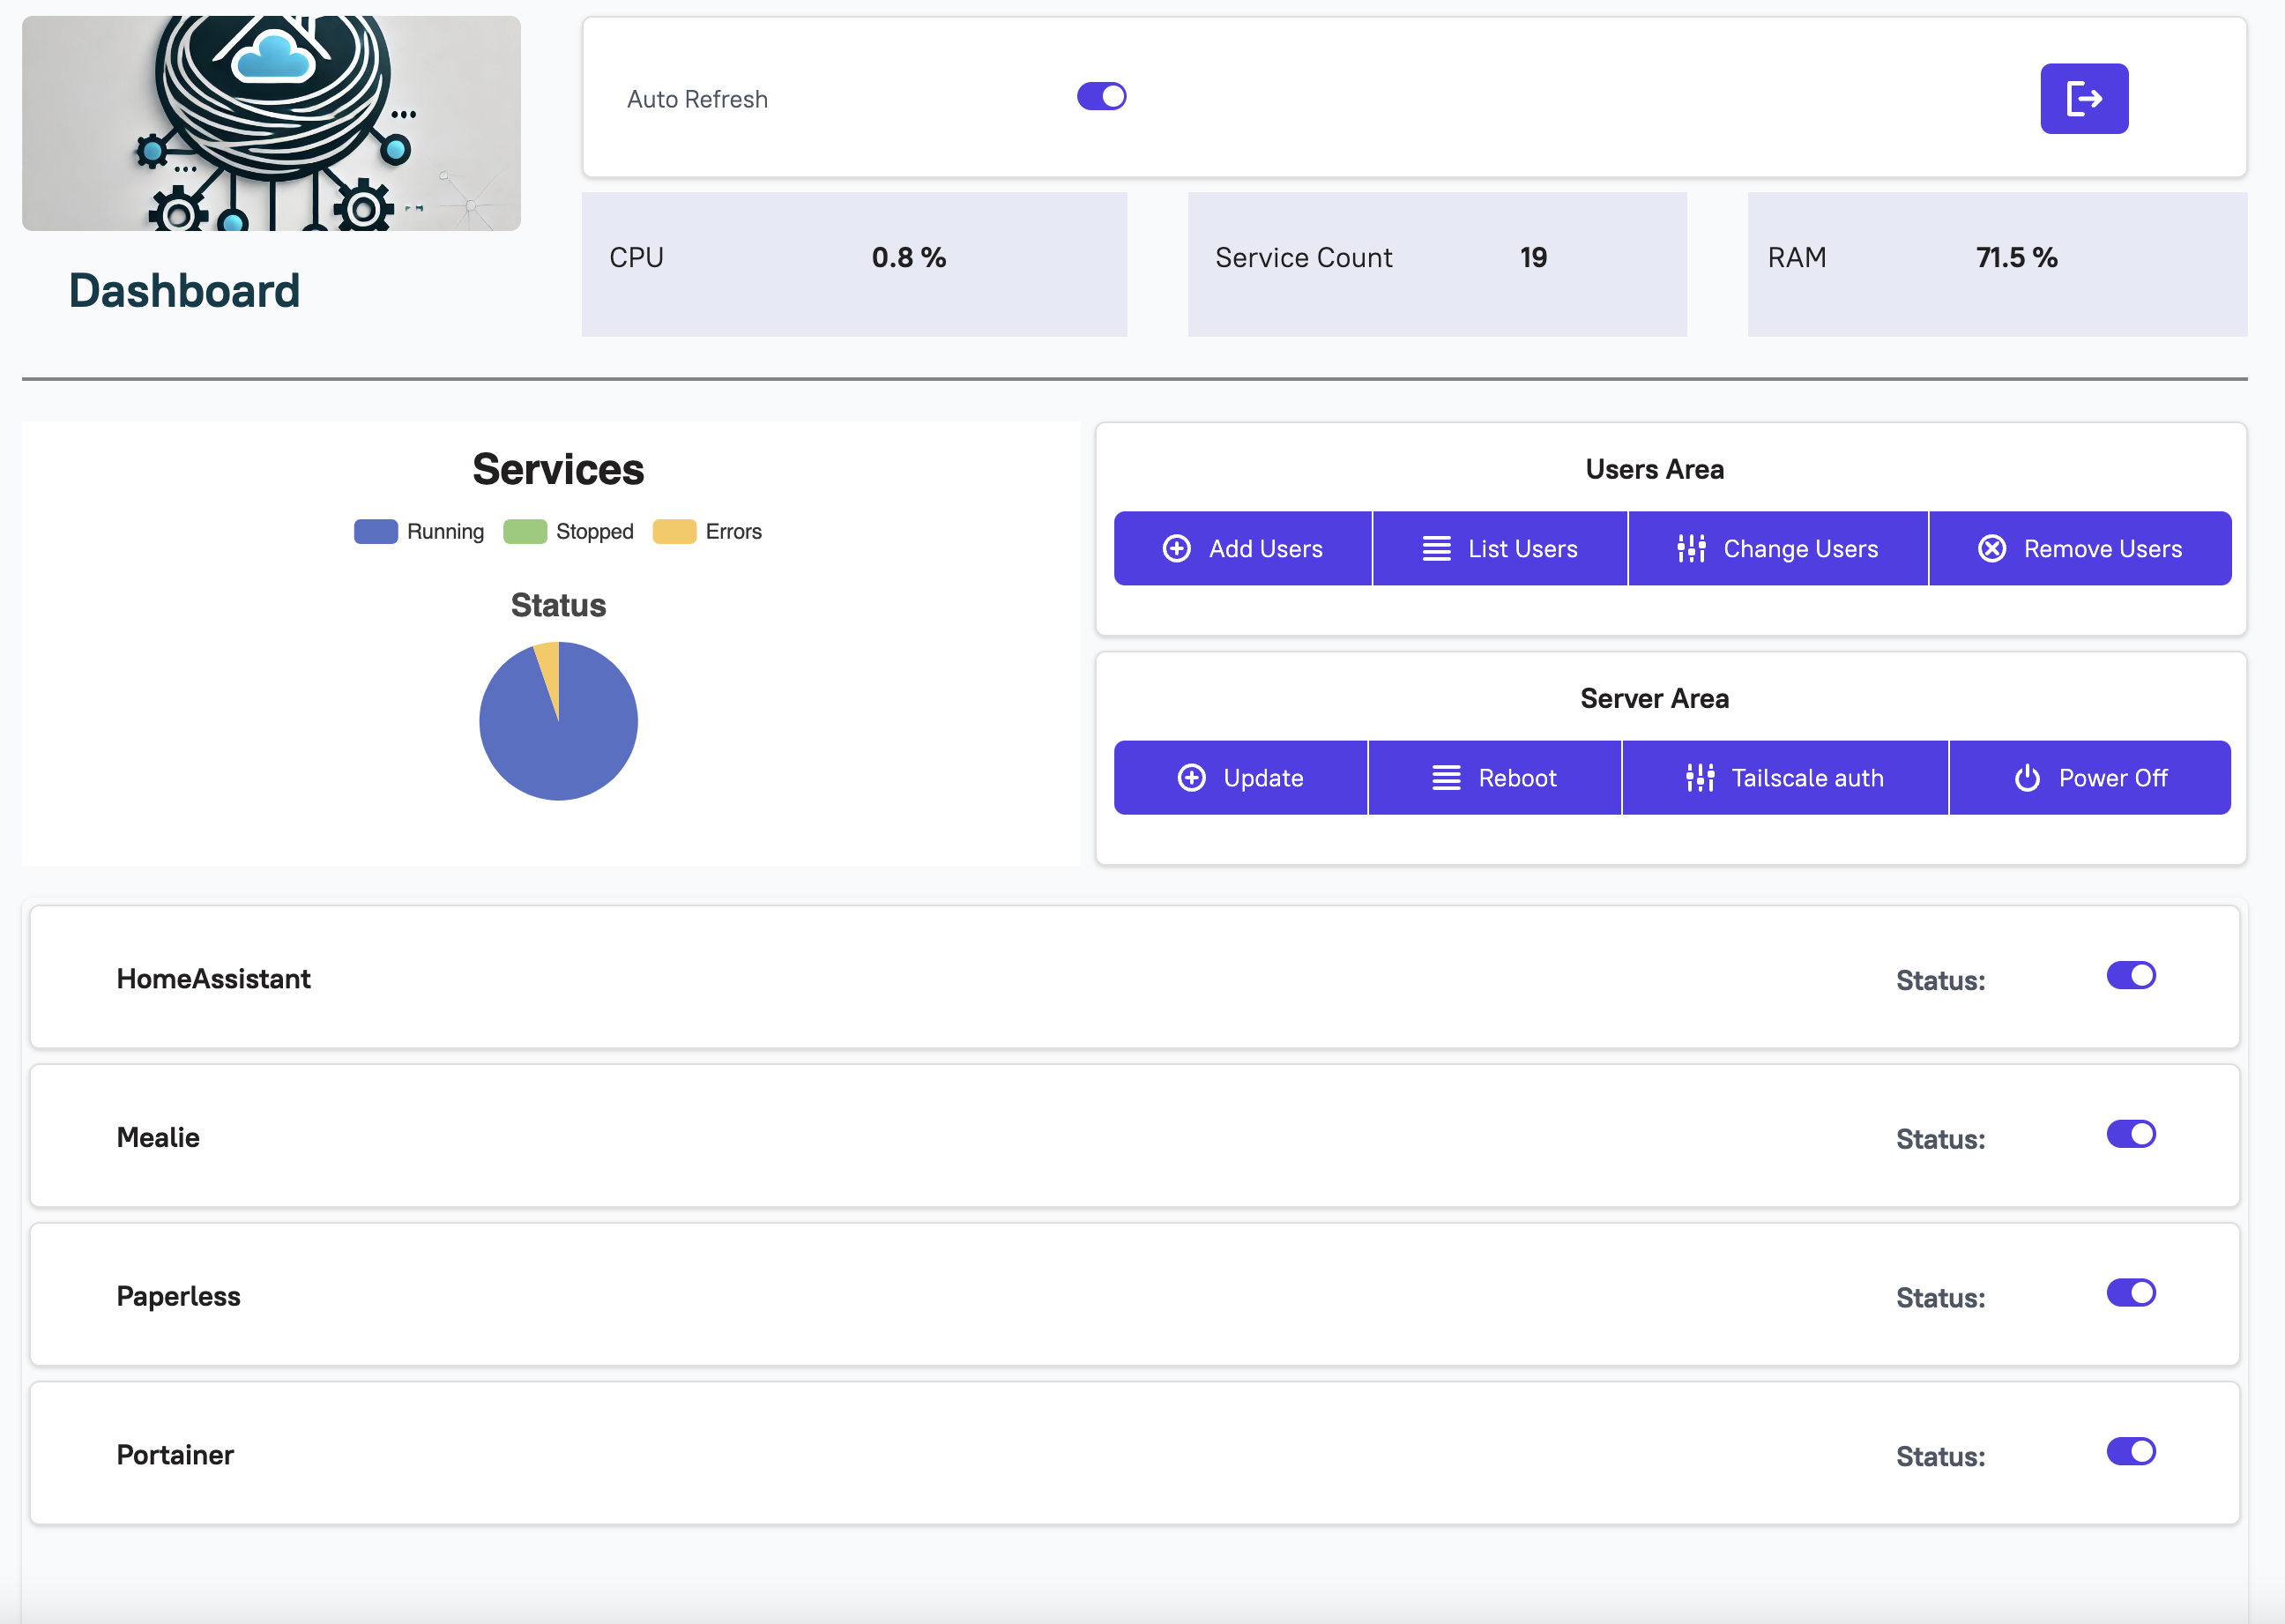
\includegraphics[width=1\textwidth]{./chapters/assets/user_interface.png}
\subsection{Projekt UI/UX}

Projektowanie interfejsu użytkownika (UI) oraz doświadczenia użytkownika (UX) odgrywa kluczową rolę w zapewnieniu funkcjonalności i intuicyjności systemu. W niniejszym rozdziale omówiono zasady projektowania UI/UX zastosowane w opracowanym interfejsie, bazując na dołączonym projekcie graficznym.

\subsubsection{Założenia projektowe}
Podstawowe cele projektowe interfejsu obejmowały:
\begin{itemize}
    \item Czytelność i prostotę obsługi,
    \item Spójność wizualną oraz intuicyjną nawigację,
    \item Minimalizację liczby kliknięć wymaganych do wykonania operacji,
    \item Odpowiednią organizację informacji w oparciu o hierarchię wizualną.
\end{itemize}

\subsubsection{Struktura interfejsu}
Projekt składa się z kilku głównych obszarów:
\begin{itemize}
    \item \textbf{Panel informacyjny} – zawierający dane dotyczące użycia zasobów systemowych (CPU, RAM, liczba usług).
    \item \textbf{Sekcja zarządzania usługami} – prezentująca status poszczególnych usług (uruchomione, zatrzymane, błędy) w formie wykresu kołowego.
    \item \textbf{Obszar użytkownika} – umożliwiający zarządzanie użytkownikami systemu (dodawanie, usuwanie, edycja).
    \item \textbf{Obszar serwera} – obejmujący podstawowe operacje administracyjne, takie jak aktualizacja systemu, restart oraz autoryzacja w Tailscale.
    \item \textbf{Lista usług} – wyświetlająca poszczególne aplikacje (np. HomeAssistant, Mealie, Paperless, Portainer) z możliwością zarządzania ich statusem poprzez przełączniki.
\end{itemize}

\subsubsection{Kolorystyka i typografia}
Projekt wykorzystuje nowoczesną, stonowaną kolorystykę z przewagą bieli i odcieni fioletu. Przyciski akcji są wyraźnie zaznaczone za pomocą intensywnych kolorów, co zwiększa ich widoczność. Tekst jest wyraźny, a hierarchia informacji zapewnia odpowiednią czytelność.

\subsubsection{Intuicyjność i użyteczność}
Projekt został zaprojektowany zgodnie z zasadami użyteczności:
\begin{itemize}
    \item Przejrzysta organizacja treści,
    \item Spójność w rozmieszczeniu elementów interfejsu,
    \item Minimalizacja zbędnych interakcji,
    \item Responsywność, umożliwiająca korzystanie na różnych urządzeniach.
\end{itemize}

Dzięki tym rozwiązaniom interfejs jest łatwy w obsłudze i spełnia wymagania użytkowników końcowych.


\subsection{Implementacja interfejsu użytkownika z wykorzystaniem podejścia no-code w Appsmith}

W celu usprawnienia procesu tworzenia interfejsu użytkownika wykorzystano platformę no-code Appsmith \cite{AppSmith}, która umożliwia szybkie budowanie aplikacji webowych za pomocą gotowych komponentów. 

\subsubsection{Proces implementacji}
Implementacja interfejsu przebiegała w kilku etapach:
\begin{enumerate}
    \item \textbf{Tworzenie struktury aplikacji} – W Appsmith utworzono nowy projekt, w którym zdefiniowano podstawowe widoki, takie jak pulpit nawigacyjny, sekcja zarządzania użytkownikami oraz obszar monitorowania usług.
    \item \textbf{Dodawanie komponentów UI} – Wykorzystano gotowe komponenty Appsmith, takie jak przyciski, tabele, wykresy i przełączniki do interakcji z użytkownikiem.
    \item \textbf{Konfiguracja źródeł danych} – Interfejs został połączony z backendem poprzez API, co pozwoliło na dynamiczne pobieranie informacji o stanie systemu i usług.
    \item \textbf{Logika aplikacji} – Za pomocą wbudowanego edytora JavaScript skonfigurowano interakcje użytkownika, m.in. obsługę formularzy, wywołania API oraz automatyczne odświeżanie danych.
    \item \textbf{Testowanie i optymalizacja} – Po wdrożeniu interfejsu przeprowadzono testy użyteczności, aby zapewnić płynne działanie aplikacji i zoptymalizować jej wydajność.
\end{enumerate}

\subsubsection{Zalety zastosowania Appsmith}
Wykorzystanie Appsmith przyniosło szereg korzyści w kontekście tworzenia interfejsu użytkownika:
\begin{itemize}
    \item Skrócenie czasu implementacji dzięki gotowym komponentom,
    \item Łatwa integracja z backendem poprzez API,
    \item Możliwość dynamicznej edycji logiki aplikacji bez konieczności pisania pełnego kodu frontendu,
    \item Prosty interfejs edytora umożliwiający szybkie wprowadzanie zmian i testowanie.
\end{itemize}

Zastosowanie podejścia no-code pozwoliło na efektywne wdrożenie interfejsu użytkownika bez konieczności zaawansowanego programowania, co znacząco przyspieszyło proces tworzenia systemu.


\section{Automatyzacja Konfiguracji i wdrozenie}

\subsection{Instalacja rozwiązania}
W ramach tworzenia rozwiązania powstał również program instalacyjny, który zostanie umieszczony na stronie internetowej rozwiązania umożliwiając pobranie przez zainteresowane korzystaniem z rozwiązania osoby.
\paragraph{Program instalacyjny}\mbox{}\\

W celu ułatwienia instalacji aplikacji na systemach użytkowników końcowych przygotowano dedykowany program instalacyjny napisany w języku Go. Aplikacja ta jest odpowiedzialna za:

\begin{itemize}
    \item Weryfikację obecności Dockera w systemie,
    \item Automatyczną instalację Dockera w systemach Linux (w pozostałych przypadkach użytkownik zostaje poinformowany o konieczności ręcznej instalacji),
    \item Pobranie najnowszej wersji aplikacji HomeNest z repozytorium GitHub,
    \item Rozpakowanie archiwum ZIP zawierającego aplikację do wskazanego katalogu,
    \item Nadanie odpowiednich uprawnień do uruchomienia aplikacji oraz jej uruchomienie.
\end{itemize}

Program wykorzystuje standardowe biblioteki Go do obsługi pobierania plików (\texttt{net/http}), rozpakowywania archiwów ZIP (\texttt{archive/zip}) oraz uruchamiania procesów lokalnych (\texttt{os/exec}). Dzięki temu działa w pełni samodzielnie, bez konieczności instalowania zewnętrznych zależności.

Logika działania programu obejmuje:
\begin{enumerate}
    \item Sprawdzenie czy polecenie \texttt{docker} znajduje się w ścieżce systemowej.
    \item Jeżeli Docker nie jest zainstalowany — uruchomienie skryptu instalacyjnego (tylko w systemach Linux).
    \item Pobranie pliku ZIP z GitHub Releases.
    \item Rozpakowanie pliku do katalogu roboczego.
    \item Uruchomienie pliku binarnego aplikacji.
\end{enumerate}

Instalator został zaprojektowany z myślą o prostocie użytkowania oraz możliwości łatwego wdrożenia aplikacji przez osoby nietechniczne. Wersje programu można przygotować na platformy Linux, Windows i macOS z wykorzystaniem narzędzia \texttt{GOOS/GOARCH}, umożliwiającego cross-kompilację.

\subsection{Integracja z narzędziami CI/CD}
\label{sec:integracja_ci_cd}

Współczesne systemy informatyczne wymagają nie tylko solidnej implementacji, ale również efektywnego zarządzania cyklem życia oprogramowania. W tym kontekście, integracja narzędzi CI/CD (Continuous Integration / Continuous Deployment) odgrywa kluczową rolę w automatyzacji procesów budowania, testowania i wdrażania aplikacji.

\subsubsection{Zastosowanie self-hosted runnera \cite{SelfHostRunner}}

W celu zapewnienia kompatybilności architektury uruchomieniowej systemu, zdecydowano się na użycie **self-hosted runnera** zamiast domyślnych runnerów GitHub Actions. Domyślne maszyny CI/CD oferowane przez GitHub działają wyłącznie na **architekturze x86**, co ogranicza możliwość testowania i wdrażania aplikacji na innych platformach, takich jak **ARM** (np. Raspberry Pi, serwery oparte na ARM64). 

Zastosowanie własnego runnera pozwala na:
\begin{itemize}
    \item Uruchamianie testów i budowanie obrazów Docker na architekturze zgodnej z docelowym środowiskiem produkcyjnym.
    \item Pełną kontrolę nad zasobami sprzętowymi wykorzystywanymi w procesie CI/CD.
    \item Możliwość integracji z lokalnym registry dla przechowywania obrazów Docker.
\end{itemize}

\subsubsection{Workflow GitHub Actions dla testowania}

\begin{verbatim}
name: Run Tests

on:
  push:
    branches:
      - main
      - dev
  pull_request:

jobs:
  test:
    runs-on: self-hosted

    services:
      mongo:
        image: mongo:latest
        ports:
          - 27017:27017

    steps:
      - name: Checkout Repository
        uses: actions/checkout@v4

      - name: Set Up Python
        uses: actions/setup-python@v4
        with:
          python-version: "3.13"

      - name: Install Dependencies
        run: |
          python -m pip install --upgrade pip
          pip install -r requirements.txt
          pip install pytest pytest-asyncio httpx

      - name: Run Pytest
        run: pytest -v
\end{verbatim}

\subsubsection{Workflow GitHub Actions dla budowania i wersjonowania obrazów Docker}

Po przejściu testów jednostkowych obraz Docker jest budowany i pushowany do lokalnego rejestru uruchomionego na **localhost:5000**.

\begin{verbatim}
name: Build and Push Docker Image

on:
    push:
      branches:
        - main
        - dev
    pull_request:
        branches: [dev, main]

jobs:
  build_and_push:
    runs-on: self-hosted

    steps:
      - name: Checkout Repository
        uses: actions/checkout@v4

      - name: Extract Version
        run: echo "VERSION=$(date +'%Y%m%d')-$(git rev-parse --short HEAD)" >> $GITHUB_ENV

      - name: Build Docker Image
        run: |
          docker build -t localhost:5000/myapp:${{ env.VERSION }} .
          docker tag localhost:5000/myapp:${{ env.VERSION }} localhost:5000/myapp:latest

      - name: Push Docker Image to Local Registry
        run: |
          docker push localhost:5000/myapp:${{ env.VERSION }}
          docker push localhost:5000/myapp:latest
\end{verbatim}

\subsubsection{Korzyści z bezpośredniego pushowania obrazu do registry}

W przeciwieństwie do wcześniejszej konfiguracji, w której obraz był zapisywany lokalnie za pomocą \texttt{docker save}, obecnie jest on od razu przesyłany do prywatnego rejestru. Takie podejście:
\begin{itemize}
    \item Umożliwia natychmiastowe wykorzystanie obrazu w środowisku produkcyjnym bez potrzeby ręcznego jego ładowania.
    \item Pozwala na prostsze zarządzanie wersjami obrazów w registry.
    \item Minimalizuje czas między budowaniem a wdrożeniem.
\end{itemize}

\subsubsection{Publikacja obrazu do lokalnego registry}

Wszystkie wersje aplikacji są automatycznie przechowywane w lokalnym rejestrze **Docker Registry**, a najnowsza wersja jest oznaczana jako \texttt{latest}. Dzięki temu wdrożenie nowej wersji sprowadza się do uruchomienia nowego kontenera:

\begin{verbatim}
docker pull localhost:5000/myapp:latest
docker run -d --name myapp localhost:5000/myapp:latest
\end{verbatim}

Dzięki temu każda wersja aplikacji jest jednoznacznie identyfikowana, a \texttt{latest} wskazuje na najnowszą stabilną wersję.